グラフ演算時にはメモリへの不規則なアクセスによるキャッシュミスが多発する.\cite{wei2016speedup} では,sd1-arc データセット (9,500万ノード,19 億エッジ)
を使用し,代表的なグラフアルゴリズムである 
Breadth-First Search (BFS) \cite{cormen2009introduction},Depth-First Search (DFS) \cite{cormen2009introduction},
Strongly Connected Component (SCC) \cite{sharir1981strong},Shortest Path (SP) \cite{cormen2009introduction},
PageRank (PR),Dominating Set (DS) \cite{cockayne1978domination},Graph Decomposition (Kcore) \cite{batagelj2003m},Graph Diameter (Diam) を
実行したところ, 演算完了までの所要時間に対し,キャッシュミス発生に伴うメインメモリアクセス時間の占める平均割合は約 70 \% であると報告されている (図 \ref{cache_miss}).
\begin{figure}[t]
  \centering
  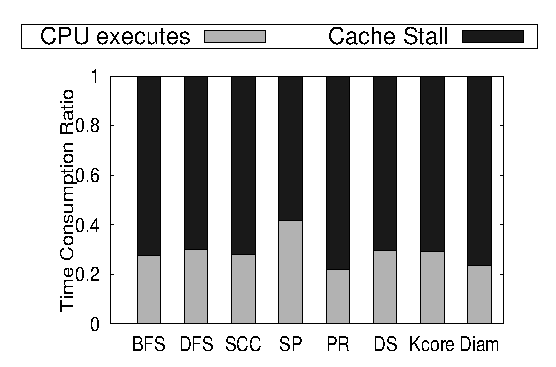
\includegraphics[scale=1.0]{./figure/cache_miss.pdf}
  \caption{CPUによる演算時間とメインメモリへのアクセス時間の比率}
  \label{cache_miss}
\end{figure}

Graph Reordering では,グラフ演算時のメモリアクセスの特徴を考慮し,ノード ID を適切に再配置することでキャッシュミス減少を実現する.
また,ノード ID の配置を変更するだけなので,グラフアルゴリズムやデータ構造自体を変更する必要はなく,既存のグラフ処理系に対して容易に適用することが可能である.

\section{グラフ演算時のメモリアクセスと ノード ID の関係}
グラフ演算において,PR での重要度や BFS での始点からの距離などのアルゴリズム固有のプロパティはノード ID をインデックス
とした配列に格納される.演算過程で隣接ノードの ID に基づき配列上で対応するプロパティを参照するという操作が繰り返され,
参照されるプロパティは CPU キャッシュへ格納される.プロパティは配列として格納されているので,ID が連続するノードのプロパティはメモリ上でも連続して
位置している.
そのため,ノード ID X のプロパティがキャッシングがされる際には,X 前後の ID を持つノードのプロパティもまとめて同一キャッシュラインに格納される.
隣接ノード群の ノード ID に連続性があるほど,キャッシング対象のライン数が減少し,ラインの入れ替え回数も減少する.
また,一般にグラフ演算はノード ID 順に行われるため,グラフ構造的に近いノードへ近いノード ID が割り振られているほど
キャッシュラインの参照回数が減少する.

\section{ID の連続性}
\section{アクセスの局所性を考慮した ID 配置}
\section{自律分散グラフ管理環境での課題}